\section{脅威モデル}
\label{sec:dns-tunneling}
本章では,はじめにDNSの概要について述べる.\\
次に,本研究における脅威モデルであるDNSトンネリングについて説明する.

\subsection{DNSの概要}
\label{sec:dns-protocol}

DNSは,IPアドレスをはじめとしたドメイン名に関連づけられたリソースレコードを解決するシステムである~\cite{rfc1034, rfc1035}.
DNSがユーザから問い合わせられたドメイン名のIPアドレスを解決してくれるおかげで,ユーザは識別しづらいIPアドレス(IPv4:``93.184.216.34", IPv6:``2606:2800:220:1:248:1893:25c8:1946")を直接入力することなく,サーバにアクセスすることができる.
このような利便性を実現するDNSによる名前解決の機能は,ユーザがインターネットを利活用する上で極めて重要である.

\subsubsection{名前空間}
DNSにおいて,各種リソースレコードが関連づけられるドメイン名は,ルートを頂点とする逆ツリー構造で構成されている.
ドメインの序列を表記する際には,上位ドメインを右に,下位ドメインを左にする.
``example.com."を例にとると,ドットで表記されるルートが最も右に位置し,ルートの一つ下層に位置するTLD(Top Level Domain)である``com"が後続する.
ドメインの区切りには,ドットが使用され,TLDの一つ下層に位置づくSLD(Second Level Domain)として``example"が連結していることを``example.com."は表しているという具合である.
図~\ref{fig:dns-architecture}に示す通り,全てのドメインには,ゾーンと呼ばれる名前空間があり,このゾーンはそれぞれのドメインに配置される権威サーバによって管理される.
DNSには,委譲という仕組みを利用することでゾーンを分割できる特徴がある.
例えば,``example"と``google"というドメインが連結している``com."について考える.
委譲の仕組みを使用しなかった場合には,``com."が``www.example.com."や``mail.google.com."といった``example.com."と``google.com."に連結した全てのドメイン名を管理する.
しかし,``com."がそれぞれのドメインにゾーンを委譲した場合,先の``www.example.com"は``example.com."が管理し,``mail.google.com."は``google.com."が管理することになる.
DNSでは,この委譲の仕組みを利用することで,ゾーンの肥大を抑止させ,サーバの負荷分散を実現する設計になっている.

\begin{figure}[h]
 \centering
 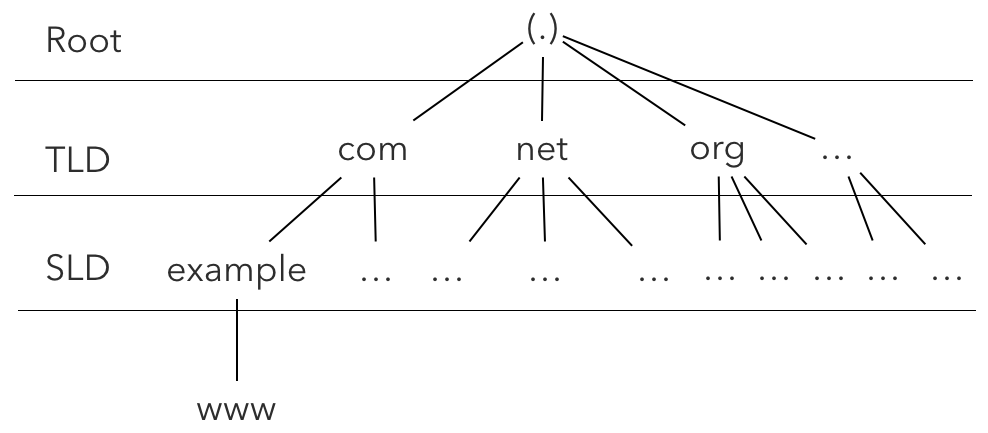
\includegraphics[width=12.0cm]{figure/dns-architecture.png}
 \caption{ドメインにおけるゾーンごとの名前空間}
 \label{fig:dns-architecture}
\end{figure}

\textbf{アーキテクチャ}\\
DNSは,クライアント・サーバアーキテクチャで構成され,機能に基づき3つのサービスに分類することができる.
\begin{itemize}
 \item スタブリゾルバ
 \vspace{-3mm}
 \item フルサービスリゾルバ
 \vspace{-3mm}
 \item 権威サーバ
\end{itemize}

スタブリゾルバは,名前解決の問い合わせるを依頼するクライアントノードである.
フルサービスリゾルバ(キャッシュサーバ・リカーシブサーバとも呼称される)は,スタブリゾルバに代わって,リソースレコードを保持する権威サーバに問い合わせるクライアントノードである.
名前解決をする際には,ルートから順にTLD,SLDという具合に権威サーバに再帰的に問い合わせることで,最終的に目的のドメイン名に関するリソースレコード情報を取得する.
この時,はじめのルート権威サーバのアドレスは``root.hints"と呼ばれるファイルに基づいて問い合わせるが,それより下位のドメインについては,上位の権威サーバが次の権威サーバのアドレスを応答することで名前解決のチェーンを繋げている.
すなわち,ルート権威サーバがTLDの権威サーバのアドレスを応答し,TLDの権威サーバがSLDの権威サーバーのアドレスを応答していく具合である.
権威サーバは,リソースレコードを保持するサーバノードであり,フルサービスリゾルバからの問い合わせ依頼に応答する.

\begin{figure}[h]
 \centering
 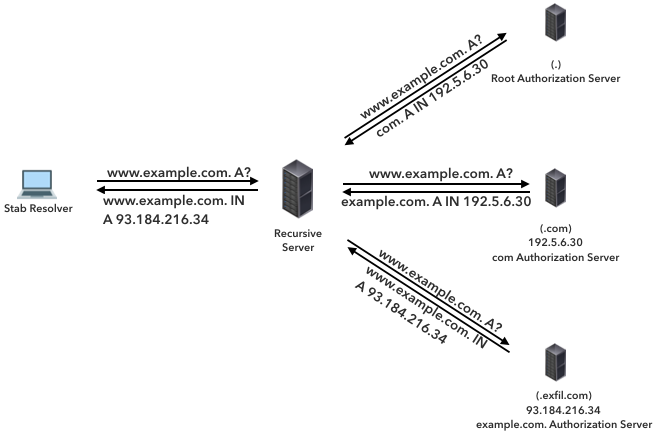
\includegraphics[width=12.0cm]{figure/dns-name-resolution.png}
 \caption{DNSによる名前解決}
 \label{fig:dns-name-resolution}
\end{figure}

\subsubsection{名前解決の仕組み}
いま,クライアントから``www.example.com"のIPv4アドレスについて問い合わせられた場合を考える.
クライアントとなるスタブリゾルバは,スタブリゾルバと同一セグメント内のフルサービスリゾルバもしくは,ネットワークセグメントに依らないパブリックなフルサービスリゾルバ(オープンリゾルバ,パブリックリゾルバとも呼称される)に問い合わせる.
フルサービスリゾルバは,その名前解決クエリが過去に解決したものでないかキャッシュデータを確認する.
キャッシュにヒットした場合にはキャッシュの情報をクライアントに応答され,ヒットしなかった場合には,root.hintsファイルを参照しルート権威サーバにリクエストパケットを転送する.
クエリ(問い合わせ)を受け取ったルート権威サーバは,``com"ドメインを委譲した権威サーバのアドレスを応答する.
次に,フルサービスリゾルバは,``com"の権威サーバに対し同じクエリを転送する.
``com"の権威サーバは,``example.com"ドメインを委譲した権威サーバのアドレスを応答する.
フルリゾルバは,``example.com"の権威サーバに同じクエリを転送する.
``example.com"の権威サーバは,保持するゾーンファイルからクエリされたドメインのリソースレコードについて探索し,探索の結果としてレコード情報をフルサービスリゾルバに応答する.
フルサービスリゾルバは,権威サーバから応答された情報をスタブリゾルバに転送することで,問い合わせられた名前は解決される.
DNSによる名前解決の一連の動作を図~\ref{fig:dns-name-resolution}で示す.

%TLDごとに登録するプロセスや必要書類,金額は異なり,上位

\subsubsection{ドメイン名とリソースレコード}
\begin{figure}[h]
 \centering
 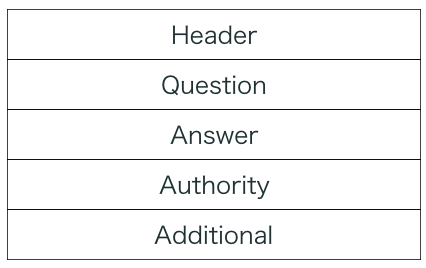
\includegraphics[scale=0.7]{figure/dns-format.png}
 \caption{DNSのパケット構造}
 \label{fig:dns-format}
\end{figure}

ドメイン名は,ルートから伸びる逆ツリー構造をドメインを表すラベルをドットで区切り表記する.
すなわち,ドメイン名は``label3.label2.label1."という具合にラベルを連結したものである.
右端のドットがルートを表現するが,全てのドメインがルートを頂点としているため,一般にルートを表す右端のドットは省略される.
図~\ref{fig:dns-format}は,DNSのパケット構造を表す.

\begin{figure}[h]
 \centering
 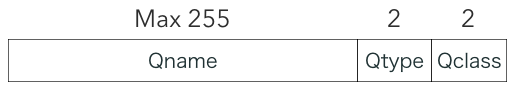
\includegraphics[scale=0.6]{figure/dns-answer.png}
 \caption{DNSのパケットのAnswerセクション}
 \label{fig:dns-answer}
\end{figure}

解決したいドメイン名は,図~\ref{fig:dns-answer}におけるQnameフィールドである.
各フィールドはサイズが決まっており,Qnameフィールドが最大長255オクテット\footnotetext{1オクテット(octet):8bit},リソースレコードのタイプを表すQtypeフィールドとクエリクラスを表すQclassフィールドがそれぞれ2オクテットである.

\begin{eqnarray}
 (LablD).(LabelC).(LabelB).(LabelA). \label{eq:domain-name} \\
 (Length) + (LabelD) + ... + (length) + (LableB) + (length) + (LabelA) + 0 \label{eq:label-name} \\ 
 1 + (Max 63) + ... + 1 + (Max 63) + 1 + (Max 63) + 1 = (Max 255) \label{eq:length-label-domain}
\end{eqnarray}

(\ref{eq:domain-name})は,複数のラベルで構成されたドメイン名の例である.
(\ref{eq:label-name})は,Questionヘッダーに注入される際のそのドメイン名を表すデータである.
Questionセクションでは,ドメイン名を表す際にドットは省略され,ラベルの長さとラベル名,そしてドメイン名の終わりを意味する``0"で表現される.
(\ref{eq:length-label-domain})は,ラベルの長さとラベル名のサイズを表す.
ラベルの長さは,8bitで表記されるため,1オクテットのサイズとなる.
ラベル長自体は,一文字が1オクテットで表され,最大長は63オクテットである.
Questionセクションの最大長255オクテットは,ラベルの長さとラベル,そしてドメイン終了を表す``0"を含めた長さである.
このため,最初のラベル長を表す1オクテットとドメイン名の終了を意味する``0"を表すための1オクテットを差し引いた253オクテットが,実際のドメイン長の最大長である.

\begin{table}[htb]
 \centering
  \begin{tabular}{ccc}
    \toprule
		\textbf{タイプ} & \textbf{値} & \textbf{意味} \\
    \midrule
    A & 1 &  ホストのIPv4アドレス \\
    NS & 2 & 権威サーバ \\
    MF & 4 & メール転送サーバ \\
    CNAME & 5 & 別名 \\
    SOA & 6 & 権威ゾーンの開始 \\
    NULL & 10 & NULL(実験用) \\
    PTR & 12 & ドメイン名のポインター(逆引き) \\
    HINFO & 13 & ホスト情報 \\
    MINFO & 14 & メールボックスおよびメールリスト情報 \\
    MX & 15 & メール交換 \\
    TXT & 16 & 任意文字列 \\
    \bottomrule
  \end{tabular}
 \caption{主要リソースレコード一覧}
 \label{tab:resource-record}
\end{table}

ラベルには,数字とアルファベットおよびハイフン(``-")を使用することができ,ラベル中に大文字・小文字の区別はない.
他方で,アルファベットなどのASCII以外にも,国際化ドメイン名(IDN: Internationalized Domain Name)を使用すると日本語やアラビア語なども使用することができる.
IDNは,Punnycodeなどのエンコーディング手法に基づき,DNSクエリする際にはASCIIコードに変換される.

ドメイン名に関連づけられる情報であるリソースレコードには複数のタイプが定義されており,目的ごとに使い分けられる.
例えば,Aというレコードタイプは,ドメイン名に対するIPv4アドレスを対応づけるために用いられる.
クライアントがあるドメイン名のIPv4アドレスが知りたいとき,スタブリゾルバは,ドメイン名とAのレコードタイプを指定することを希望のIPv4アドレスを取得することができる.
表~\ref{tab:resource-record}は,主要なリソースレコードである.


%リソースレコードのタイプごとの使用頻度を知りたい
% タイプごとの説明を充実させるのは,重要かもしれない


\subsection{DNSトンネリング}
%DNSトンネリングが脅威となりうる点に関する説明
%概念
DNSトンネリングは,DNSをデータ転送のメディアとした秘匿通信手法の総称であり,転送元と転送先の方向性によって二つに分類することができる.
一つ目がDNS Exfiltrationと呼ばれる,スタブリゾルバから権威サーバ方向へのデータ転送手法であり,二つ目がDNS Infiltrationと呼ばれ,権威サーバからスタブリゾルバ方向へのデータを転送手法である.
%DNSトンネリングという手法は,ポートスキャンで知られるNmapのメーリングリストだとされている.
DNSトンネリングは,以下に示すDNSの特性に基づいた秘匿手法である.

\begin{itemize}
 \setlength{\itemsep}{0pt}
 \item インターネットを利用する際にDNSを用いた名前解決をする必要があり,ほとんどの組織でポートが閉ざされることが少ない
 \item 通常インターネットを利用する度にDNSクエリが発生するため,クエリログは肥大化しやすく長期のログ保存が困難である
 \item 任意の文字列を注入できるフィールドを保持している
 \item 正規のDNSクエリとDNSトンネリングによるDNSクエリのパケットの違いは,Qnameフィールドに含まれる文字列のみに現れるため,100\%の精度で分類することが困難である
\end{itemize}

以上のようなDNSの特徴を利用することで,DNSトンネリングは秘匿通信として機能する.
DNSトンネリング手法が脅威なのは,IDS・IPSなどの検知システムにフィルタリングされにくく,クエリ頻度を長期化させた場合解析を迂回することができる点である.
DNSトンネリングがデータ転送のキャリアとするフィールドは,クエリのQuestionセクションのQnameと,AnswerセクションのRdataである.
QuestionセクションのQnameフィールドを利用することで,スタブリゾルバから権威サーバ方向にデータを転送できる.
この方向の通信は,ビーコン通信やターゲットから取得した情報を外部に漏えいさせるといった攻撃の最終目的を達成するのに使われる.
また,AnswerセクションのRdataフィールドを利用することで,権威サーバからスタブリゾルバ方向にデータを転送することができる.
この方向の通信は,ターゲットネットワーク内のホストに潜伏したマルウェアなどへの命令コードを送信するのに使われる.
さらに,この二つのキャリアを利用することが双方向の通信路を確保できるため,C2通信を実施することも可能である.

DNSトンネリングの手法は,ポートスキャンで知られるNmapのメーリングリストにて初めて一般に公開された(1998年)~\cite{nmap}.
その後,多くのDNSトンネリング実装~\cite{ozymandns, iodine, dnscat2, tcp-over-dns, dnscat, denise, dns-shell, dnsbotnet, dnscapy, dohtunnel, godoh, dohc2, magictunnelandroid}が公開され,実際の攻撃シーンへの転化されるに至る.


\subsubsection{スタブリゾルバから権威サーバ方向}
\label{sec:dns-exfiltration}

\begin{figure}[h]
 \centering
 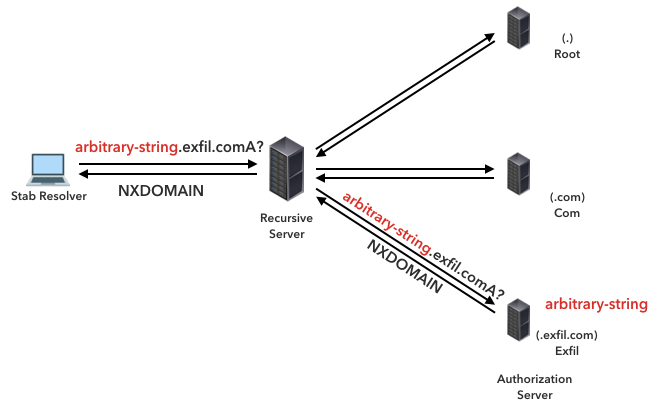
\includegraphics[width=12.0cm]{figure/dns-exfiltration.png}
 \caption{arbitrary-stringという任意の文字列が,DNSクエリのラベル部を用いて,事前に用意した権威サーバ(exfil.com)に転送される様子}
 \label{fig:dns-exfiltration}
\end{figure}

DNS Exfiltrationは,再帰問い合わせの仕組みによって,DNSクエリがコンテンツを保持する権威サーバに転送される仕組みをを利用した手法.
これによって,クライアントから権威サーバを宛先とする方向に対して任意のデータを転送することができる.
データを転送するためのキャリアは,DNSクエリのQuestion SectionのQNAME内のラベルである.
第~\ref{sec:dns-protocol}節で示すように,ドメイン名には一つのラベルあたり63byte,全体で253bitという制約がある.
すなわち,DNS Exfiltrationによって転送できるデータ量の最大は253byteである.
他方で,DNSの名前解決の仕組みはインターネットの利活用において必要不可欠であるため,多くの組織においてDNSのトラフィックがフィルタリングされることはほとんどない.
このような性質をもつDNSを利用することで,悪意を持つユーザがなんらかの方法で潜伏した組織内部rネットワークから情報を流出させる際の手法として,他のネットワークプロトコルに比べて都合が良い.

DNS Exfiltrationにおいて,データを転送する際の宛先ノードは特定のゾーンを管理する権威サーバである.
例えば,あるローカルネットワーク内に位置づくノードからグローバルネットワーク内の``exfil.com"という権威サーバにデータを転送することを考える.
一般に,転送するデータをQNAMEにおけるラベルに埋め込む際には,Base Encoding~\cite{rfc4648}のような変換規則によるエンコード処理が施される.
この処理によって,転送データがバイナリデータである際にも転送効率上げたり,ラベルの文字列制約を満たさないデータも転送することができる.
また,メッセージの意味抽出を困難にするためのトリックとして用いられる.
変換された文字列は,


この権威サーバは,``exfil.com"以下の全ての名前空間をゾーンとして管理することができる.
データを転送する際のキャリアとなるのは,DNSクエリの``exfil.com"以下のラベルである.
DNSのラベルは,数字・アルファベット・先頭以外でハイフン(``-")という文字列の制約があるため,任意の文字列をそのまま注入することは困難である.
任意の文字列を文字列エンコーディングの手法で変換させ,用意できた文字列をQNAMEに含め,適当なリソースレコードタイプを指定すれば,宛先となる権威サーバにデータが転送される.
最後に,ラベルを同一の文字列エンコーディングアルゴリズムでデコードすることで,元のデータを受け取ることができるという具合である.
このようにして,DNSの名前解決の仕組みを応用することで,任意の権威サーバに任意の文字列を転送することができる.
これがDNS Exfiltrationの動作メカニズムである.
図~\ref{fig:dns-exfiltration}に,DNS Exfiltrationのメカニズムを図解した様子である.


%1998年4月,DNSトンネリングの手法は,NmapのBugtraqメーリングリストにて初めて公になったとされている\cite{bugtraq}.

\subsubsection{権威サーバからスタブリゾルバ方向}
\label{sec:dns-infiltration}

\begin{figure}[h]
 \centering
 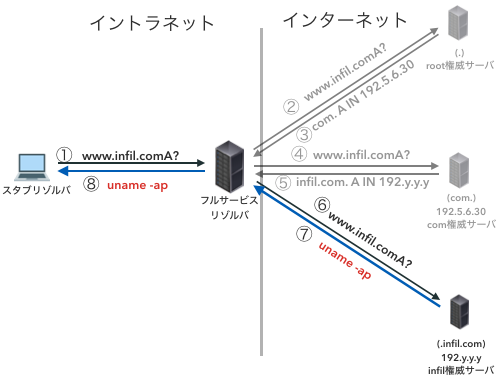
\includegraphics[width=10.0cm]{figure/dns-infiltration.png}
 \caption{TXTレコードに登録された情報について,DNSクエリで問い合わせることで権威サーバから命令情報を取得している様子}
 \label{fig:dns-infiltration}
\end{figure}

DNS Infiltrationは,DNS Exfiltrationと逆方向の権威サーバからクライアント方向にデータを転送する手法である.
この手法は,DNSのリソースレコードに任意の文字列が含められる設計になっていることを利用したものである.
リソースレコードのタイプは多種多様であるが,ゾーンファイルを自由に編集できる現在のDNSエコシステムでは,ドメイン名との関わりに関係なく任意の情報をドメイン名に関連づけることが可能である.
DNS Infiltrationを実施するには,送信元となる権威サーバのドメイン名に,適当なリソースレコードのタイプ(E.g. TXT)に転送したい文字列を登録しておくことで,そのドメイン名をQNAMEとしてそのレコードタイプを問い合わせることで,クライアントのもとでデータを回収することができるという具合である.
DNSのリソースレコードを転送キャリアとする流入通信のメカニズムを図解した様子が,図~\ref{fig:dns-infiltration}である.


% Null タイプは,厳密に定義されておらず,実験用としか表現されていない.しかし,全体のタイプのうち,20%を示す程度に頻繁に使用されるタイプのである.

\subsection{検知に基づく既存対策手法}
本節では,DNSトンネリングに対するこれまでの対策手法について説明する.
% 検知に基づく手法の現在までの程度を淡々と示す.
\subsubsection{特徴量}
DNSトンネリングの手法を用いる場合,いくつかの特徴が現れることがある.
Bornら~\cite{born}は,DNSトンネリングにおけるクエリ内のドメイン名に出現する文字の出現頻度を着目
することで,正規のドメイン名とDNS Exfiltrationメソッドによって生成されたドメイン名とを分類のに有用であることを明らかにした(2010).
著者らは,正規のドメインであれば英語のような自然言語における文字の出現頻度と高い相関があることに加えて,エントロピーと文字列分布に高い相関があることも明らかにした.


\subsubsection{閾値推定}
\subsubsection{機械学習に基づくモデル}
%\subsubsection{パターンマッチング}
%\subsubsection{同一ドメインあたりのクエリ頻度}
%\subsubsection{Qnameにおける文字列分布}
%\subsubsection{Qnameにおける長さとエントロピー}
%\subsubsection{課題 : Low ThroughputなTunnelingに対する検知手法}
DNSトンネリングメソッドを使用した時のDNSクエリは,で述べるような特性が出現する.
この性質に基づき,これまでに多数の検知手法が提案されてきた.
